\lab{Algorithms}{Numerical Derivatives}{Numerical Derivatives}
\label{Ch:Numerical Derivatives}

\objective{Understand and implement finite difference approximations of the derivative. Then explore Image Filters. In particular, we will explore the Sobel Filter, which uses 
numerical derivatives to find edges in images.}

\section*{One Dimension}

The derivative of a function at a point is formally defined as

\begin{equation}
\label{eqn:deriv}
f'(x) = \lim_{h\rightarrow 0} \frac{f(x + h)-f(x)}{h}.
\end{equation}

In most real world applications we will be solving problems using computers. How does a computer calculate a limit? In short it can't. Computers can only approximate functions at specific points, and the notion of a limit graces infinity in a way that a computer never can.

So how can we use a computer to find the derivative of a function, particularly when we can't differentiate the function by hand? We use methods known as finite difference methods. For example suppose that in equation \ref{eqn:deriv}, instead of taking a limit we just pick a particularly small value for h. Then we have

\begin{equation*}
f'(x) \approx \frac{f(x + h)-f(x)}{h}
\end{equation*}

This is known as the first order forward difference approximation of the derivative.

How do we know the quality of this approximation? We can use Taylor's formula to find

\begin{equation*}
f(x_0 + h) = f(x_0) + hf'(x_0) + h^2/2 f''(\xi),\hspace{5mm} \xi \in (x_0,x_0 + h)
\end{equation*}

Which can be also expressed as

\begin{equation*}
f'(x_0) = \frac{f(x_0 + h) - f(x)}{h} + \frac{h}{2}f''(\xi) = \frac{f(x_0 + h) - f(x)}{h} + O(h)
\end{equation*}

Here we use the big-O notation to denote that the errors are bounded by some constant multiplied by $h$.

We can use Taylor expansions to find approximations that have different big-O error bounds, up to any polynomial of arbitrary degree. Tables \ref{Table:CDiff} and \ref{Table:FDiff} offer the coefficients for centered and forward difference schemes.

\begin{table}
\begin{center}
\begin{tabular}{|c|c|c|c|c|c|c|c|c|}
\hline
Derivative & Accuracy & -3 & -2 & -1 & 0 & 1 & 2 & 3 \\ \hline
 & 2 & & & -1/2 & 0 & 1/2 & & \\ \cline{2-9}
 1 & 4 & & 1/12 & -2/3 &  0 & 2/3 & -1/12 & \\ \cline{2-9}
  & 6 & -1/60 & 3/20 & -3/4 & 0 & 3/4 & -3/20 & 1/60 \\ \hline
  & 2 & & & 1 & -2 & 1 & & \\ \cline{2-9}
 2 & 4 & & -1/12 & 4/3 &  -5/2 & 4/3 & -1/12 & \\ \cline{2-9}
  & 6 & 1/90 & -3/20 & 3/2 & -49/18 & 3/2 & -3/20 & 1/90 \\ \hline
\end{tabular}
\caption{Centered Difference Coefficients}
\label{Table:CDiff}
\end{center}
\end{table}

\begin{table}
\begin{center}
\begin{tabular}{|c|c|c|c|c|c|c|}
\hline
Derivative & Accuracy & 0 & 1 & 2 & 3 & 4 \\ \hline
 & 1 & -1 & 1 &  & &  \\ \cline{2-7}
 1 & 2 & -3/2 & 2 & -1/2 & &  \\ \cline{2-7}
  & 3 & -11/6 & 3 & -3/2 & 1/3 &  \\ \hline
  & 1 & 1 & -2 & 1 &  & \\ \cline{2-7}
 2 & 2 & 2 & -5 & 4 &  -1 &  \\ \cline{2-7}
  & 3 & 35/12 & -26/3 & 19/2 & -14/3 & 11/12 \\ \hline
\end{tabular}
\caption{Forward Difference Coefficients}
\label{Table:FDiff}
\end{center}
\end{table}

These tables can be used by simply summing the function evaluations (the number at the top represents how many times $h$ is added to $x$), and then dividing by $h^n$, where $n$ is the degree of the derivative.

So, for example, the centered difference estimate of the second derivative that is $O(h^4)$ is
\begin{equation*}
f''(x) \approx \frac{-1/12(f(x-2h) + f(x+2h)) + 4/3(f(x-h) + f(x+h)) -5/2f(x)}{h^2}
\end{equation*}

Or, the forward difference estimate for the first derivative that is $O(h^2)$ is

\begin{equation*}
f'(x) \approx \frac{-3/2f(x) + 2f(x+h) - 1/2 f(x+2h)}{h}
\end{equation*}

It should be noted that we can convert a forward difference estimate to a backwards difference estimate by using $-h$. So the backwards difference estimate for the first derivative that is $O(h^2)$ is

\begin{equation*}
f'(x) \approx \frac{3/2f(x) - 2f(x-h) + 1/2 f(x-2h)}{h}
\end{equation*}

There are two important observations that you should make about these tables. First, in order to get higher order approximations we need to evaluate the function at more points. This should not be surprising. Second, you should notice that centered difference formulas require less function evaluations to get higher order approximations. However, in certain applications it is not possible to use centered difference formulas, so the backwards and forwards formulas are still very applicable.

One important aspect of this method is selecting an appropriate $h$. The natural temptation is to pick a very very small value. However, this is not always advisable. Note the values in table \ref{Table:FloatingError}, which approximates the derivative of $e(x)$ at $x = 1$:

\begin{table}[h!]
\begin{center}
\begin{tabular}{|cc|}
\hline
h & Error  = $|f'(1)-f'_{app}(1)|$ \\ \hline
1e-1 & 4.5e-3 \\
1e-3 & 4.5305e-7 \\
1e-7 & 5.8587e-11 \\
1e-10 & 6.7274e-7 \\ \hline
\end{tabular}
\caption{Error in numerical derivative, using double precision floating point arithmetic}
\label{Table:FloatingError}
\end{center}
\end{table}

As you can see, the error actually increases as $h$ becomes very small. Why is this? Division by small numbers causes errors in floating point arithmetic. So, be aware that usually the optimal $h$ is of moderately small size. However, in the framework of double floating point arithmetic, this is usually less of a concern.

As a matter of reference, calculating numerical derivatives is an unstable operation. An unstable operation, informally, is one where errors are magnified by the operation. This usually is not an issue, but it's important to know that taking derivatives can amplify errors.

\begin{problem}
Write a function \li{numDer1} that accepts as inputs: a callable function object \li{f} and
a keyword argument \li{h} giving the step size (default \li{h = 1e-5}). Have the function return an array of the approximate 1st order derivative with accuracy 1 of \li{f} at each of the points in \li{pts}, using the centered  coefficients.
\end{problem}

\begin{problem}
Write a function \li{numDer2} that accepts as inputs: a callable function object \li{f} and
a keyword argument \li{h} giving the step size (default \li{h = 1e-5}). Have the function return an array of the approximate 2nd order derivative with accuracy 1 of \li{f} at each of the points in \li{pts}, using the centered  coefficients.
\end{problem}

\begin{comment}
\begin{problem}
Write a function \li{numDer} that accepts as inputs: a callable function object \li{f}, an
array of numbers \li{pts}, a keyword argument \li{mode} (taking one of the values 
\li{'centered'}, \li{'forward'}, or \li{'backward'}), a keyword argument \li{d} (taking one of 
the values \li{1} or \li{2}), a keyword argument \li{o} (taking an integer value in 
\li{[2, 4, 6]} if \li{mode = 'centered'}, and otherwise taking a value in \li{[1, 2, 3]}), and
a keyword argument \li{h} giving the step size. The default settings of the keyword
arguments should be \li{mode = 'centered', d = 1, o = 2, h = 1e-5}.
 
Have the function return an array of the approximate derivative of order \li{d} with accuracy
 \li{o} of \li{f} at each of the points in \li{pts}, using the coefficients indicated by \li{mode}.
\end{problem}
\end{comment}

We note that higher order approximations of the derivative can be derived using the Taylor series and Lagrange polynomials, but generally higher-order approximations are not practically useful as they can often be ill-conditioned.

For any numerical approximation method, it is important to be able to empirically calculate
the order of convergence. We will do so for our numerical derivative approximation. 
For an $m$-th order approximation of the first derivative, we have that the error is in
$O(h^m)$, so that
$$
err(h) \approx Ch^m
$$
for some constant $C$.
Hence, taking the log of both sides, we obtain
$$
\log err(h) \approx \log C + m\log h,
$$
which means that if we plot the log of the errors against the log of the $h$ values, we 
ought to see a linear relationship whose slope gives the rate of convergence. 

We do this in python as follows (The \li{numDer} function in this code can use any of the coefficients from \ref{Table:CDiff} and \ref{Table:FDiff}):
\begin{lstlisting}
# assume that the function numDer has already been written
import numpy as np
from matplotlib import pyplot as plt

# approximate the derivative of cosine at x = 3
# create a callable function object
def myCosine(x):
    return np.cos(x)
f = myCosine

# calculate the actual derivative
actual = -np.sin(3.0)

# initialize array of h values at which to calculate the error
hvals = np.linspace(1e-5, 1e-1)
err1 = np.zeros(hvals.shape)
err2 = np.zeros(hvals.shape)

# calculate the errors for order 1 and order 2 approximations for the forward coeffiects
for i in xrange(len(hvals)):
    err1[i] = np.abs(actual - numDer(f, np.array([3.0]), mode = 'forward', h = hvals[i], o=1))
    err2[i] = np.abs(actual - numDer(f, np.array([3.0]), mode = 'forward', h = hvals[i], o=2))

# plot the log of the h values against the log of the errors
plt.subplot(121)
plt.loglog(hvals, err1)
plt.ylim((1e-11, 1e-1))
plt.subplot(122)
plt.loglog(hvals, err2)
plt.ylim((1e-11, 1e-1))
plt.show()
\end{lstlisting}

The generated plot is shown in Figure \ref{fig:convergence}. Note that the slope
of the line in the left plot is about 1, and the slope of the line in the right
plot is about 2. Further, the log of the errors for the order 2 approximations
are much lower than the log of the errors of the order 1 approximations.

\begin{figure}[t]
    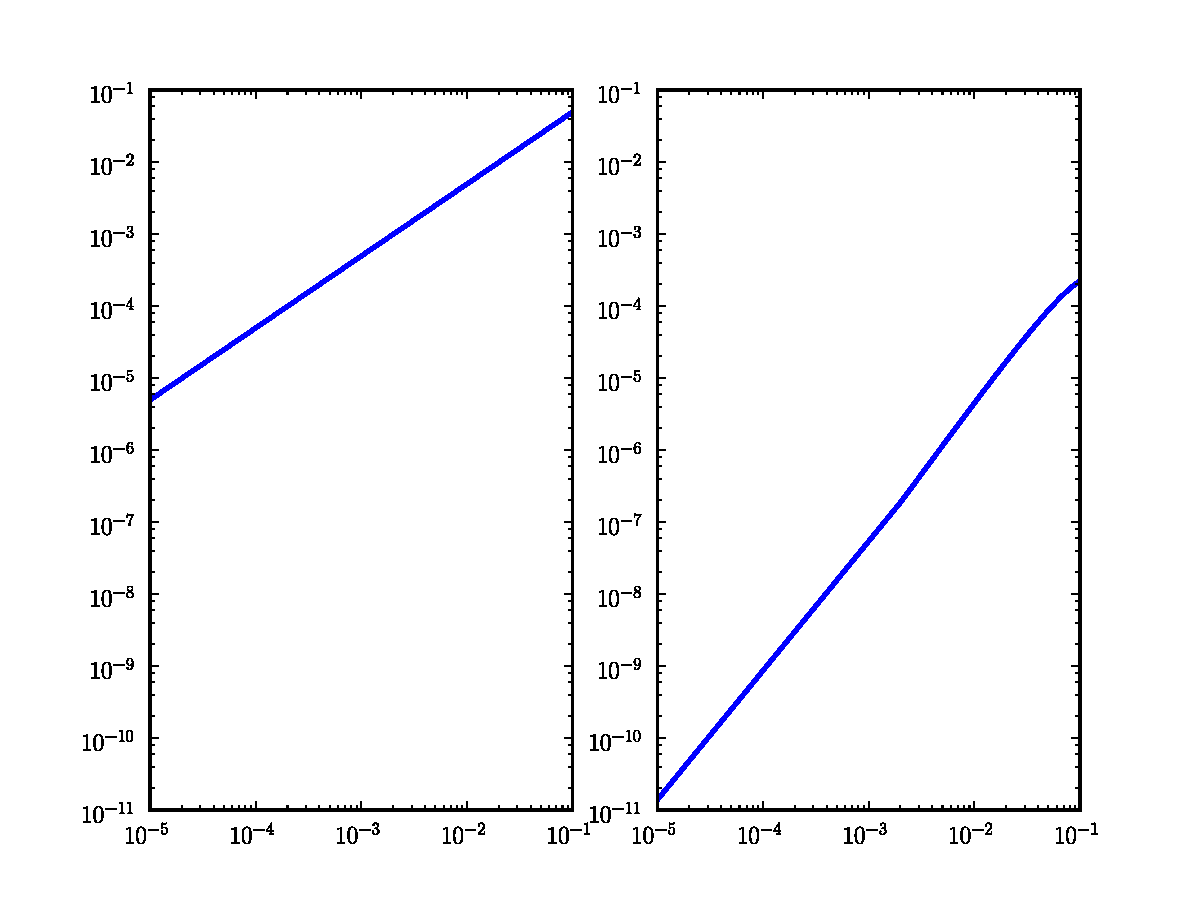
\includegraphics[width=0.8\textwidth]{convergence.pdf}
    \caption{Convergence plots for our numerical derivative approximations.
    The left plot shows the convergence for order 1 approximations. 
    The right plot shows the convergence for order 2 approximations.}
    \label{fig:convergence}
\end{figure}

\begin{comment}
\begin{problem}
Explore the convergence properties for different orders of approximation,
and for the second derivative as well. You may need to adjust your $h$
values, as they may be too small for some of the calculations.
\end{problem}
\end{comment}

\section*{Multi Dimensions}

The Jacobian is a generalization of the derivative in many dimensions. We can think of it, 
intuitively, as defining a linear approximation to the function in a neighborhood of some given
point. If the function happens to be real-valued, the Jacobian defines a tangent plane to the graph of 
the function at a point. 
The Jacobian is of critical importance in a variety of areas, and we will use it in lab \ref{lab:NewtonsMethod}
to find zeros of multivariate functions.

Formally, the Jacobian of a function $f:\mathbb{R}^n \rightarrow \mathbb{R}^m$ is an $m \times n$ matrix. It is defined by the formula:
\begin{equation*}
J_{ij} = \frac{\partial f_i}{\partial x_j}
\end{equation*}

We can use finite difference approximations to find partial derivatives in the natural manner:
\begin{equation*}
\frac{\partial f}{\partial x_i} (x) \approx \frac{f(x+h e_i)-f(x)}{h}
\end{equation*}
where $e_i$ is a unit vector in the $i$th coordinate (the direction $x_i$). Higher order approximations and centered and backwards differences follow by naturally extending this definition.

\begin{problem}
Write a function \li{Jacobian} that accepts a function handle, an integer giving the dimension of the
range of the function, an integer giving the dimension of the domain of the function, a NumPy array giving
the point at which to approximate the Jacobian, and an optional argument giving the step size $h$. Use center approximation of order 1.
Return a NumPy array giving the approximated Jacobian matrix at the given point.

If the function under consideration maps from $\mathbb{R}^n$ to $\mathbb{R}^m$, the function handle should
accept as input an array of shape \li{(n,)} and return an array of shape \li{(m,)}.

Test your function on the following $f: \mathbb{R}^2 \to \mathbb{R}^2$:
\begin{equation*}
f(x, y) =
\begin{pmatrix}
e^{x} \sin(y) + y^3 \\
3y - \cos(x)
\end{pmatrix}
\end{equation*}

Compare your \li{Jacobian} function against the analytically computed derivative on the square $[-1,1] \times [-1,1]$ using ten thousand grid points (100 per side). Which method is faster? What is the maximum error of your function?
\end{problem}

Given a function from $\mathbb{R}^n \to \mathbb{R}$, sometimes the mixed partial derivatives are useful. In particular, the mixed partials will be useful when we study optimization in Volume 2. This information is contained in the Hessian matrix, which is defined as

\begin{equation*}
H_{ij} = \frac{\partial^2 f}{\partial x_i \partial x_j}
\end{equation*}

We can use the following formula to approximate mixed partial derivatives
\small
\begin{equation*}
\frac{\partial^2 f}{\partial x_i \partial x_j} = \frac{f(x + (e_i + e_j)h) - f(x + (e_i-e_j)h) -f(x + (e_j-e_i)h) + f(x - (e_i + e_j)h)}{4h^2}
\end{equation*}
\normalsize

\begin{problem}
Write a Python function that numerically calculates the Hessian of a given function. 
The function should be named \li{Hessian}, and should accept as inputs a function handle, 
an integer giving the dimension of the domain of the function, a NumPy 
array giving the point at which to approximate the Hessian, and an optional argument giving the 
step size.
Return the approximated Hessian matrix at the given point.

Test it on the following function
\begin{equation*}
f(x,y) = (1-x)^2 + 100(y-x^2)^2
\end{equation*}
This function is known as the Rosenbrock Banana function, or Rosenbrock's Valley. It is a common test function for optimization algorithms because it is non-convex and the global minimum is hard to find from certain starting points. A graph is shown in figure \ref{Fig:Rosenbrock}. Compare the output of your function with the analytic solution on the region $[-2,2] \times [0,2]$, using ten thousand points. What is the maximum error of your function?
\end{problem}
\begin{figure}
\begin{center}
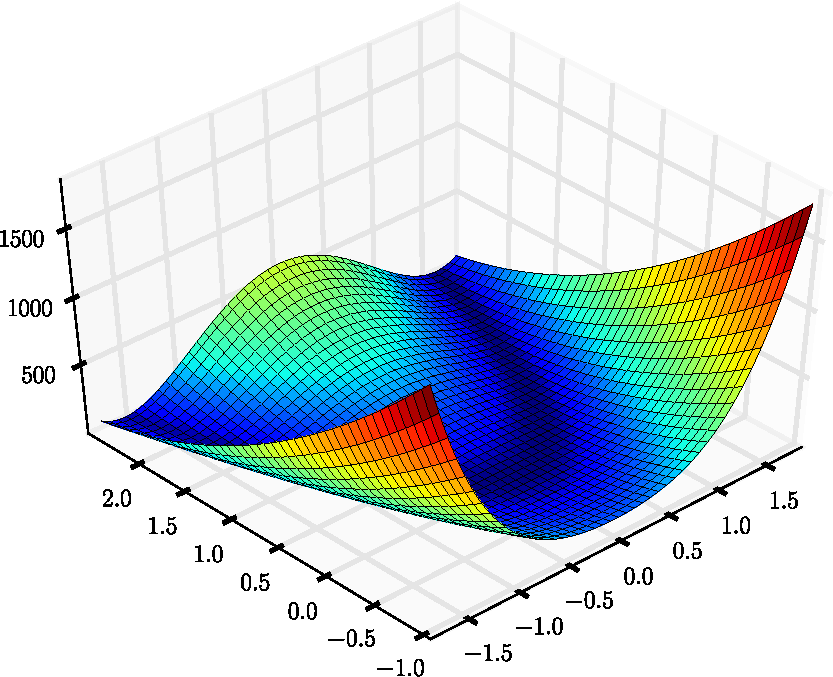
\includegraphics[width = \textwidth]{Rosenbrock}
\caption{The Rosenbrock Banana Function, a common test function in optimization algorithms}
\label{Fig:Rosenbrock}
\end{center}
\end{figure}

\section*{Application: Image Filters}
One of the primary tools in image processing is the use of filters to identify important information 
in images. In this section we will implement our own filters and explore applications.

One of the easiest filters to implement is matrix based. In this implementation, the filter that we 
select is a matrix, which represents how much we want certain pixels to contribute to the output image. 
Suppose that we choose our filter to be:

\[
A = \begin{pmatrix}
a_{-1,-1}&a_{-1,0}&a_{-1,1}\\
a_{0,-1}&a_{0,0}&a_{0,1}\\
a_{1,-1}&a_{1,0}&a_{1,1}
\end{pmatrix}.
\]

We will call our input image $B$ and our output image $C$ (both images are represented as matrices).
Our matrix filter operates according to the following formula:
\[
C_{ij} = \sum_{k=-1}^1 \sum_{m=-1}^1 a_{km}B_{i+k,j+m}.
\]

Essentially this computes each pixel of the output image as the weighted sum of the surrounding
pixels in the input image. The technical term for this type of operation is a convolution.

Suppose that our image $B$ is an $m\times n$ matrix. Note that the definition for
$C_{ij}$ given above does not make sense when $i = 0, m-1$ or $j = 0, n-1$, since we would be trying
to access matrix elements $B_{-1,j}, B_{m,j}, B_{i,-1},$ or $B_{i,n}$, which are out of bounds.
%One fix is to treat these out-of-bounds elements as copies of the nearest in-bounds element.
%That is, define
%\begin{align*}
%B_{-1,j} &:= B_{0,j},\\
%B_{m,j} &:= B_{m-1,j},\\
%B_{i,-1} &:= B_{i,0},\\
%B_{i,n} &:= B_{i,n-1}.
%\end{align*}
%For the corners, define
%\begin{align*}
%B_{-1,-1} &:=B_{0,0},\\
%B_{m,-1}&:= B_{m-1,0},\\
%B_{-1,n}&:=B_{0,n-1},\\
%B_{m,n}&:=B_{m-1,n-1}.
%\end{align*}
One fix is to assign the value of 0 to these out-of-bounds elements. This process is know as \emph{padding}
the image with zeros. The amount of padding necessary is dependent on the size of the filter.
In the following code, we create a padded version of the image $B$ with respect to a filter $f$ of shape 
$h\times k$, where we assume that $h$ and $k$ are odd integers.

\begin{lstlisting}
>>> import numpy as np
>>> # assume that the matrix B and filter f already exist.
>>> # create padded version of B.
>>> m, n = B.shape
>>> h, k = f.shape
>>> B_pad = np.zeros((m + h - 1, n + k - 1))
>>> B_pad[h/2:h/2 + m, k/2:k/2 + n] = B
\end{lstlisting}

We can now easily calculate a given element of the filtered image $C$ as follows:
\begin{lstlisting}
>>> C[i,j] = (f*B_pad[i:i + h, j:j + k]).sum()
\end{lstlisting}

Make sure that you understand why this Python code does what we want it to do.
\begin{problem}
Write a function \li{Filter} that takes an image and an arbitrary filter matrix, and outputs the
filtered image. Note that for these filters to be meaningful, the number of columns and number 
of rows need to be odd (there are ways to deal with even size filters, but we won't handle them here).
\end{problem}

So what can we do with these filters? We will show an example of how to apply a Gaussian blur 
using this type of filter. You will also be able to test your code with this example. 
To begin, load the following picture:

\begin{lstlisting}
>>> import numpy as np
>>> from matplotlib import pyplot as plt
>>> K = plt.imread('cameraman.tif')
>>> plt.imshow(K, cmap = plt.cm.Greys_r)
>>> plt.show()
\end{lstlisting}

This code should display an image like the one shown in Figure \ref{imfil:camclean} (provided
that you have the correct image file, of course).

\begin{figure}
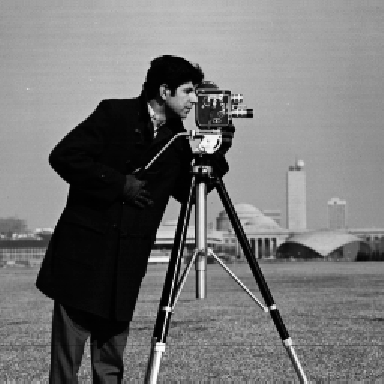
\includegraphics{cameramanClean.pdf}
\caption{An example image.}
\label{imfil:camclean}
\end{figure}

Now that you have a simple filter function, try the following filter on this image:

\[
A = \frac{1}{159}\begin{pmatrix}
2&4&5&4&2\\
4&9&12&9&4\\
5&12&15&12&5\\
4&9&12&9&4\\
2&4&5&4&2
\end{pmatrix}
\]

\begin{lstlisting}
>>> A = np.array([[2,4,5,4,2],
                 [4,9,12,9,4],
                 [5,12,15,12,5],
                 [4,9,12,9,4],
                 [2,4,5,4,2]])/159.
>>> C = Filter(K, A)
>>> plt.imshow(C, cmap = plt.cm.Greys_r)
>>> plt.show()
\end{lstlisting}
You should get an output that looks something like Figure \ref{imfil:camblur}.
\begin{figure}
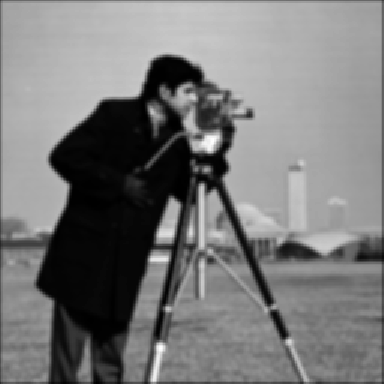
\includegraphics{cameramanBlur.pdf}
\caption{A blurred version of Figure \ref{imfil:camclean}.}
\label{imfil:camblur}
\end{figure}
You can see that the filter blurred the image. This can be very important in trying to 
wash out images that are ``noisy.''

We now turn our attention to the problem of edge detection. Automatically detecting edges in an image
can be useful in segmenting the image, detecting and extracting certain features in the image, and
sharpening contrast in the image. There are many approaches to this problem, and in this lab, we will
design a filter that numerically approximates the gradient of the image at each pixel. The magnitude
of the gradient tells us the local rate of change of the pixel values, and so large magnitudes 
correspond to regions of high contrast in the image. Since there is high contrast at edges within
the image, we have reason to hope that this approach will be effective.

The filter we will use is called the \emph{Sobel Filter}. To find the gradient 
in the vertical direction, the filter is given by:
\[
A = \frac{1}{8}\begin{pmatrix}
-1&-2&-1\\
0&0&0\\
1&2&1
\end{pmatrix}
\]
The filter for the horizontal gradient is simply the transpose of the above matrix.

For an image $B$, suppose that filtered images using the Sobel filter in the vertical and
horizontal directions are given by $B_y$ and $B_x$, respectively. These two matrices give
the $y$ and $x$ components of the gradient, respectively, at each pixel. To obtain the 
magnitude of the gradient (i.e. the length of the gradient vector), we use the formula
$$
B_{grad} = \sqrt{B_x^2 + B_y^2},
$$
where the square root and squaring operations are performed pointwise on the matrices. 
The matrix $B_{grad}$ now gives the magnitude of the gradient at each pixel, and so we
can threshold this matrix to isolate the pixels with the largest gradient, setting all 
other pixel values to 0. 
In Python, this can be done as follows:
\begin{lstlisting}
>>> B_edges = B_grad > thresh
\end{lstlisting}
where \li{thresh} is some positive threshold value of our choosing. In general, a reasonable
value for this threshold is $4\mu(B_{grad})$, where $\mu(B_{grad})$ is the mean value of the 
matrix $B_{grad}$.
If we now plot the matrix \li{B_edges}, we will see a black-and-white image with the edges 
shown as white lines.

\begin{problem}
Write a function \li{plotEdges} that finds and plots the edges of an image using the Sobel filter.
The function should take an image, and the last line of code should be a call 
to \li{plt.show}. The function should not return anything. For your threshold value, use the 
suggestion given above.

For the cameraman example, you should obtain an output similar to that displayed in 
Figure \ref{imfil:edges}.
\end{problem}

\begin{figure}[h!]

\includegraphics{edges.pdf}
\caption{A filtered version of Figure \ref{imfil:camclean}.}
\label{imfil:edges}
\end{figure}


